\subsection{Subclasses Do Not Redefine Methods}
    \textit{Subclasses Do Not Redefine Methods} (\textit{SR}), definito da M. Lippert et al. \cite{lippert2006refactoring}, afferma che se le sottoclassi non ridefiniscono i metodi delle loro superclassi può essere indice del fatto che attraverso l'ereditarietà non è espressa nessuna astrazione ma è più che altro ereditarietà implementativa \cite{lippert2006refactoring}.
        %è uno \textit{smell} definito da M. Lippert e S. Roock \cite{lippert2006refactoring} \cite{SURYANARAYANA201521} che si verifica quando una sottoclasse non ridefinisce nessun metodo della sua superclasse. 
        
    Questo può essere indice del fatto che attraverso la gerarchia non è espressa nessuna astrazione e che non c'è quindi alcun motivo per cui questa gerarchia debba essere presente nel design. 
    La presenza di questo \textit{smell} può essere causata principalmente dalla tendenza all'utilizzo delle gerarchie per il riutilizzo delle funzionalità del padre, senza però che la classe e il suo supertipo condividano una relazione IS-A. 
    
    \paragraph{Nodo di tipo smell nel grafo}
    Il nodo dello \textit{smell} SR dispone di due o più archi in uscita verso altrettante \textit{unit}: 
    \begin{itemize}
        \item Presenta la dipendenza \textit{affects} verso la \textit{unit} colpita dallo \textit{smell}.
        
        \item È in relazione con almeno una \textit{unit} attraverso un arco di tipo \textit{fatherInvolved}, che indica i supertipi della classe che presenta lo \textit{smell}.
    \end{itemize}
    
    %Problemi e refactoring
    \subsubsection{Impatto sulla qualità del codice e refactoring}
        %La presenza di questo smell può influenzare diversi aspetti riguardanti la qualità del codice \cite{SURYANARAYANA201521}, come  comprensibilità, riusabilità, facilità nella modifica ed estensione, affidabilità sono tutti affetti negativamente dalla presenza di \textit{Subclasses Do Not Redefine Methods}. 
        La presenza di \textit{Subclasses Do Not Redefine Methods} può influenzare in maniera negativa la qualità del codice attraverso la compromissione di proprietà quali comprensibilità, riusabilità, facilità nella modifica, estensione e affidabilità \cite{SURYANARAYANA201521}.
        
        Analizzando nel dettaglio le qualità influenzate negativamente dalla presenza di questo \textit{smell}, si può affermare che:
        \begin{itemize}
            \item Quando le classi in una relazione gerarchica non condividono una relazione concettuale IS-A, può portare a molta confusione e ridurre la \textit{comprensibilità} del sistema, confondendo gli sviluppatori e i progettisti.
            
            \item Se le \textit{unit} non condividono una relazione IS-A il riutilizzo del codice potrebbe essere compromesso poiché non è possibile la sostituzione delle istanze dei sottotipi con i loro supertipi. Questa situazione renderebbe difficile il \textit{riutilizzo} dell'intera gerarchia in un altro contesto. Questo potrebbe causare diversi problemi ulteriori relativi alla difficoltà nella \textit{modifica ed estensione} della gerarchia, poiché un cambiamento potrebbe avere un grosso impatto sul codice.
            
            \item La presenza di classi che non condividono una relazione IS-A potrebbe portare a diversi problemi di \textit{affidabilità} del codice, poiché lo scambio tra un'istanza di una superclasse con quella di una sottoclasse potrebbe causare errori indesiderati.
        \end{itemize}
        
        Per il \textit{refactoring} di questo \textit{smell} l'applicazione di \textit{Replace Inheritance With Delegation} è la scelta consigliata e più diffusa \cite{SURYANARAYANA201521}. Questa strategia consiste nella trasformazione della relazione IS-A tra le due classi in una relazione di utilizzo, in modo che la ex-sottoclasse abbia al suo interno un oggetto dell'altra per l'utilizzo dei suoi metodi.
        
        % Considerazioni sullo smell (esempio cosa dell'overloading - già approfondita sopra - , )
    
    %Strategie di identificazione
    \subsubsection{Strategia di identificazione}
        Devo controllare che in ogni relazione gerarchica presente nel programma analizzato non si verifichi la ridefinizione di almeno un metodo del supertipo da parte del sottotipo. Per fare questo, è necessario controllare che l'intersezione dei metodi definiti dalle due classi sia vuota e quindi non abbiano almeno un metodo in comune. 
        Nella ricerca dei metodi definiti dalla superclasse viene utilizzata la funzione \textit{getAllMethods} definita in precedenza poiché, se i metodi delle interfacce non fossero considerati, una situazione analoga a quella definita dalla figura 2, dove il sottotipo (nodo beige) ridefinisce un metodo (nodo verde) definito solamente dall'interfaccia (nodo azzurro) ma non implementato dalla classe astratta (nodo rosso), verrebbe considerata come \textit{smell}. È stato deciso però di non ritenere questa situazione come tale poiché le due classi condividono una relazione IS-A e il metodo dell'interfaccia che la classe concreta implementa è derivato comunque dal suo supertipo.
        %i metodi che la classe astratta può anche non implementare sono stati considerati come fossero \textit{abstract}, ridefiniti poi dalle classi concrete che la estendono.
        \defaultvspace
        \begin{figure}[h]
            \centering
            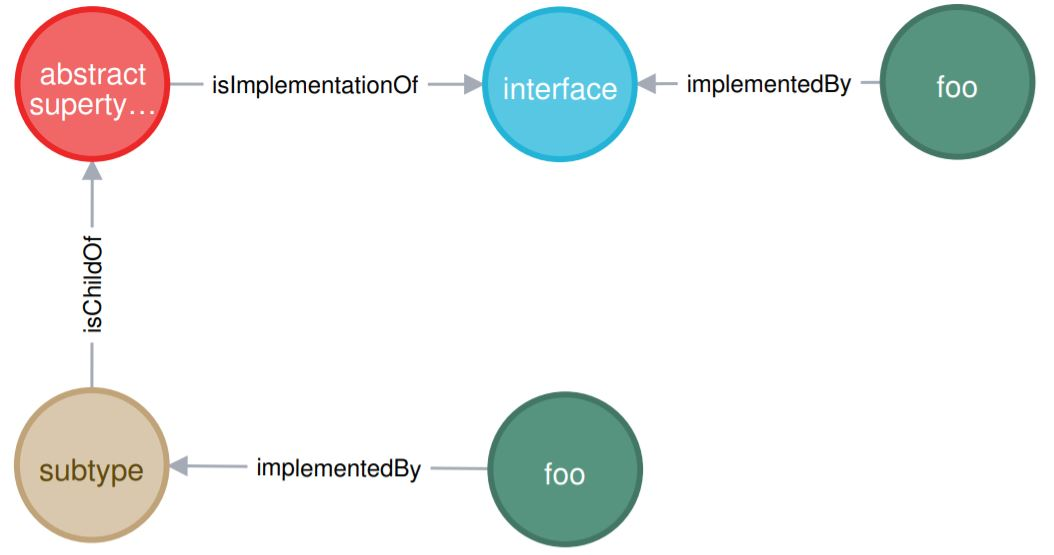
\includegraphics[scale=0.5]{Tesi/Sezione3-RiconoscimentoSmell/immagini/grafo1.JPG}
            \caption{Esempio interfaccia implementata da una classe astratta}
            \label{fig:my_label}
        \end{figure}
        \defaultvspace \\
        %Dalle relazioni considerate vengono escluse però quelle gerarchiche tra due interfacce, p
        %Per l'identificazione di questo smell inoltre non sono state considerate due diverse categorie di unit:
        Dalle relazione \textit{isChildOf} considerate vengono escluse tutte quelle che coinvolgono:
        \begin{itemize}
            \item Due \textit{unit} \textit{interface}, poichè nelle gerarchie tra interfacce non avviene la ridefinizione di metodi ma si verifica solamente l'estensione del comportamento attraverso nuove funzioni, pertanto tutti questi casi risulterebbero falsi positivi.
            
            \item Una \textit{unit} di tipo classe che rappresenta una \textit{exception} (oppure anche \textit{error}), poiché è molto comune che abbiano come supertipo una \textit{exception} e richiamino solamente il costruttore utilizzando parametri diversi. In questi casi non c'è ridefinizione dei metodi ma non è stato giudicato comunque come \textit{smell}, in quanto la relazione IS-A è presente.
        \end{itemize}
        %
        % tutte le coppie di nodi di tipo classe che condividono una relazione \textit{isChildOf} dove
        In termini di grafo è necessario considerare tutti i nodi che presentano un arco \textit{isChildOf} in uscita dove almeno un nodo di tipo \textit{function} in ingresso al nodo considerato non condivida la proprietà \textit{name} con un'altro nodo \textit{function}:
        \begin{itemize}
            \item Definito da uno dei supertipi della classe analizzata, dove per supertipi si intendono i nodi che hanno in ingresso gli archi \textit{isChildOf} provenienti dalla classe sotto analisi.
            
            \item Presente nella gerarchia di uno dei supertipi. Per verificare questo si seguono tutti gli archi \textit{isChildOf} e \textit{implementedBy} a partire dai supertipi al fine di controllare anche tutti i metodi ereditati.
        \end{itemize}
        %In termini di grafo bisogna considerare tutte le coppie di nodi di tipo classe che condividono una relazione isChildOf dove il nodo del supertipo non ha in ingresso un nodo function che condivide il nome con almeno un nodo function che la unit padre ha in ingresso. 
        %Inoltre è necessario risalire la gerarchia seguendo le relazioni \textit{isChildOf} per verificare che il sottotipo non abbia un nodo function 
        %Inoltre è necessario anche risalire la gerarchia della classe padre per verificare che il sottotipo non ridefinisca qualche metodo che il padre erediti dalla sua gerarchia, poichè il parser delle funzioni non include nella unit eventuali metodi ereditati. DA MIGLIORARE LE InFo sUL GRAFO
        
    
    %Algoritmo
    \subsubsection{Algoritmo}
        \paragraph{Input} un sottografo del grafo principale, considerando solamente i nodi che rappresentano classi (concrete e astratte) coinvolte in una dipendenza del tipo \textit{isChildOf} e le relative funzioni definite dalle classi. Oltre all'arco \textit{isChildOf} sarà considerato anche \textit{implementedBy}.
        %Gli archi considerati sono invece di tipo \textit{isChildOf} e \textit{implementedBy}
    
        \paragraph{Output} una lista di classi che presentano lo \textit{smell} e i relativi supertipi coinvolti.
        
        \paragraph{Algoritmo}
            \begin{algorithmic}
    \Function{Subclasses-does-not-redefine-methods-detector}{ }
        \State{Prendo tutti i nodi che hanno almeno un arco in entrata del tipo}
        \State{isChildOf, escludendo le interfacce e le enumerazioni}
        \For{Ogni vertice trovato, che rappresenta il supertipo}
            \State{Prendo la lista delle funzioni definite ed ereditate dalla unit,}
            \State{includendo anche quelli definiti dalle interfacce implementate}
            \If{La lista dei metodi considerata non è vuota}
                \For{Ogni sottotipo con isChildOf in uscita verso il supertipo}
                    \State{Prendo la lista di tutte le funzioni definite dal sottotipo}
                    \If{L'intersezione tra le liste dei metodi è l'insieme vuoto}
                        \State{Aggiungo il vertice alla lista degli smell}
                    \EndIf
                \EndFor
             \EndIf
        \EndFor
    \EndFunction
\end{algorithmic}
    
